\documentclass{article}%
\usepackage[T1]{fontenc}%
\usepackage[utf8]{inputenc}%
\usepackage{lmodern}%
\usepackage{textcomp}%
\usepackage{lastpage}%
\usepackage{booktabs}%
\usepackage{hyperref}%
\usepackage{lipsum}%
\usepackage{microtype}%
\usepackage{nicefrac}%
\usepackage{url}%
\usepackage{bookmark}%
\usepackage{tabularx}%
\usepackage{svg}%
%
\title{Report Example}%
\author{Insert Author Name here}%
\date{25/09/2019}%
%
\begin{document}%
\normalsize%
\maketitle%
\section{Introduction}%
\label{sec:Introduction}%
This is a sample introduction. 
\lipsum[1-2]
\linebreak%
\newline%
\linebreak%
\section{Data}%
\label{sec:Data}%
Insert your text here.%
\lipsum[1]%
\linebreak%
\newline%
\linebreak%
\subsection{Linear Regression}%
\label{subsec:Linear Regression}%
We can perform a simple linear regression with one of the 
variables against the response factor.
Here we use sklearn's LinearRegression model.\\
The variable we are using is the age. 

\begin{figure}[!ht]%
\centering%
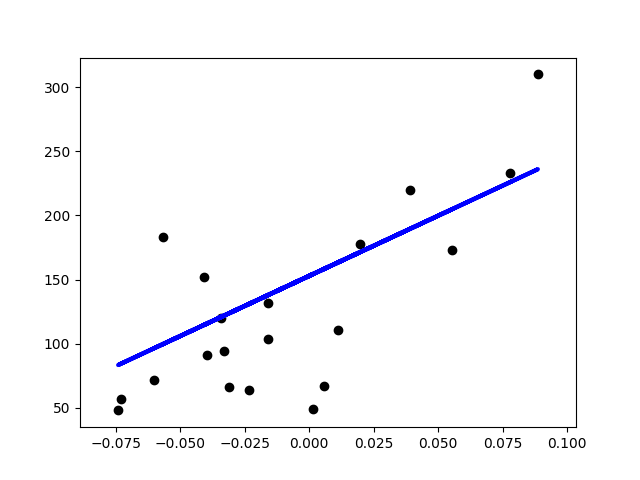
\includegraphics[scale=0.6]{../figures/Figure1.png}%
\linebreak%
\caption{This is a plot of the linear reg output. This plot was saved to a random directory and copied to the 'figures' folder of this report.}
\end{figure}
\\    
\begin{tabular}{llr}
\toprule
{} &             Results &  Values \\
\midrule
0 &      Coefficient(s) &     938 \\
1 &  Mean Squared Error &    2548 \\
2 &      Variance Score &       0 \\
\bottomrule
\end{tabular}
\\\caption{Results of the Logisitic Regression}


\lipsum[5]
%
\newline%
\linebreak%
\section{Conclusion}%
\label{sec:Conclusion}%
Insert your text here.%
\lipsum[1]%
\linebreak
%
\newline%
\linebreak%


\begin{figure}[!ht]%
\centering%
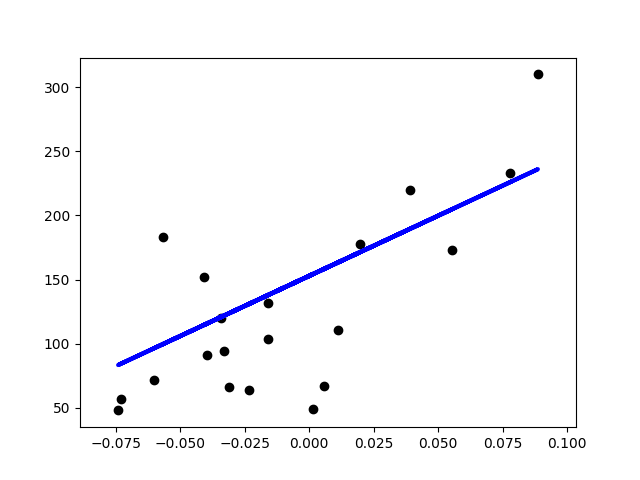
\includegraphics[scale=0.6]{../figures/Figure1.png}%
\linebreak%
\caption{This is a plot of the linear reg output.}%
\end{figure}

%
\newline%
\linebreak%


\begin{figure}[!ht]%
\centering%
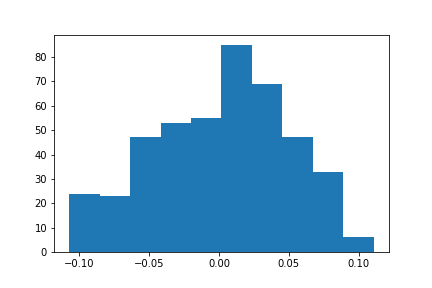
\includegraphics[width=0.5\textwidth]{../figures/Figure2.png}%
\linebreak%
\caption{This is a histogram of the patients' age.}%
\end{figure}

%
\newline%
\linebreak%
\begin{center}\begin{tabular}{llr}
\toprule
{} &             Results &  Values \\
\midrule
0 &      Coefficient(s) &     938 \\
1 &  Mean Squared Error &    2548 \\
2 &      Variance Score &       0 \\
\bottomrule
\end{tabular}
\end{center}\\\centerline{\caption{Results of the Logisitic Regression}}%
\newline%
\linebreak%
\begin{center}\begin{tabular}{lrrrrrrrrrr}
\toprule
{} &    age &    sex &    bmi &     bp &     s1 &     s2 &     s3 &     s4 &     s5 &     s6 \\
\midrule
count & 442.00 & 442.00 & 442.00 & 442.00 & 442.00 & 442.00 & 442.00 & 442.00 & 442.00 & 442.00 \\
mean  &  -0.00 &   0.00 &  -0.00 &   0.00 &  -0.00 &   0.00 &  -0.00 &   0.00 &  -0.00 &  -0.00 \\
std   &   0.05 &   0.05 &   0.05 &   0.05 &   0.05 &   0.05 &   0.05 &   0.05 &   0.05 &   0.05 \\
min   &  -0.11 &  -0.04 &  -0.09 &  -0.11 &  -0.13 &  -0.12 &  -0.10 &  -0.08 &  -0.13 &  -0.14 \\
25\%   &  -0.04 &  -0.04 &  -0.03 &  -0.04 &  -0.03 &  -0.03 &  -0.04 &  -0.04 &  -0.03 &  -0.03 \\
50\%   &   0.01 &  -0.04 &  -0.01 &  -0.01 &  -0.00 &  -0.00 &  -0.01 &  -0.00 &  -0.00 &  -0.00 \\
75\%   &   0.04 &   0.05 &   0.03 &   0.04 &   0.03 &   0.03 &   0.03 &   0.03 &   0.03 &   0.03 \\
max   &   0.11 &   0.05 &   0.17 &   0.13 &   0.15 &   0.20 &   0.18 &   0.19 &   0.13 &   0.14 \\
\bottomrule
\end{tabular}\end{center}
\\\centerline{\caption{Descriptive table of diabetes data.}}%
\newline%
\linebreak%
\begin{tabular}{lrrr}
\toprule
{} &     s1 &     s3 &     s5 \\
\midrule
count & 442.00 & 442.00 & 442.00 \\
mean  &  -0.00 &  -0.00 &  -0.00 \\
std   &   0.05 &   0.05 &   0.05 \\
min   &  -0.13 &  -0.10 &  -0.13 \\
25\%   &  -0.03 &  -0.04 &  -0.03 \\
50\%   &  -0.00 &  -0.01 &  -0.00 \\
75\%   &   0.03 &   0.03 &   0.03 \\
max   &   0.15 &   0.18 &   0.13 \\
\bottomrule
\end{tabular}
\\\caption{Merged dataframes example.}%
\newline%
\linebreak%
\clearpage%
\end{document}